\cotefile{14}
\scanpage{117}
\uline{Notations} \quad Pour $X$ variété projective non singulière.
\[
\left\{\begin{aligned}
&H^{*}(X).\quad \text{cohomologie $\unsure{l|\ell}$-\unsure{adiques|adique}}\\
&P^{*}(X)\quad \text{Partie primitive de la cohomologie}
\end{aligned}\right.
\]
\margin{on peut mettre des coeff.}

\diagram{\(\left\{\begin{array}{ll}
 A^{*}(X)=A^{*}_{r}(X)&\text{anneau de Chow (équiv. rationnelle)}\\
 N^{*}(X)=A^{*}_{a}(X)&\text{\qquad \textquotedblleft\qquad pour équiv. algébrique}\\
 J^{*}(X)=A^{*}_{r}(X)^{a}&\\[4pt]
 \multicolumn{2}{l}{\begin{tikzcd}[ampersand replacement=\&,column sep=small]
 0\arrow[r]\&J^{*}(X)\arrow[r,dash]\&A^{*}(X)\arrow[r]\&N^{*}(X)\arrow[r]\&0
 \end{tikzcd}}
 \end{array}\right.\)}

\[
\left\{\begin{aligned}
M^{*}(X)&\quad\text{partie primitive de }N^{*}(X)\\
I^{*}(X)&\quad\text{partie primitive de }J^{*}(X)
\end{aligned}\right.
\]

\uline{N.B.} Il ne semble pas qu'il y ait une définition raisonnable de la \textquotedblleft partie primitive\textquotedblright\ de $\unsure{A^{*}|A|N^{*}|\mathcal A^{*}}(X)$ \ldots

% archive sheet number: 116
\scanpage{118}
1) Les cycles num. équivalents à $0$ sur $X$, mod équiv. rationnelle, sont décrits par un nb fini de \textquotedblleft familles algébriques\textquotedblright\ de cycles.
\[
\Longrightarrow\left\{\left(\begin{aligned}
&\text{équiv. num.}=\tau\text{-équivalence}\\
&\text{les } A^{i}_{a}(X)\text{ sont de type fini......}
\end{aligned}\right)\right.\quad\Downarrow
\]

2) \(\displaystyle (x,y)-(x,b)-(a,y)+(a,b)\underset{a}{\sim}0\)

\[
1),\ \text{et }2)\quad\Longrightarrow\quad\text{Les }A^{i}_{r}(X)^{a}\text{ sont des V.A.}
\]
\[
\left\{\begin{aligned}
A^{i}_{r}(X)^{a}\times A^{d}_{r}(\deleted{X}Y)^{a}&\unsure{\relbar|\longrightarrow}A^{i+d}_{r}(X\times Y)^{a}\quad\text{est nul}\\
A^{i}_{r}(X)^{a}\times A^{d}_{r}(X)^{a}&\relbar A^{i\unsure{+|-}\unsure{j|d}}_{r}(X)^{a}\quad\text{est nul}
\end{aligned}\right.
\]
\[
\begin{aligned}
\deleted{\unsure{1)\Rightarrow}}&\qquad A_{0}^{\deleted{\unsure{*|i}}}(X)^{a}\xrightarrow{\sim}\operatorname{Alb}(X)\qquad\text{bijectif}\\
2)\Longleftrightarrow&\qquad A_{0}(X\times Y)^{\unsure{a|\cdot}}\overset{\sim}{\relbar}A_{0}(X)^{a}\times A_{0}(Y)^{a}\quad\text{bijectif}
\end{aligned}
\]

% archive sheet number: 117
\scanpage{120}
$X$ schéma projectif
\[
M\subset K(X)
\]
\uline{Conditions équivalentes} \quad (i) $\exists$ familles \uline{limitées} de faisceaux \inserted{loc. libres} $(F_i)(G_i)$ sur $X$, tel que $M$ contenu ds l'ens des
\[
\gamma(F_i)-\gamma(G_i)
\]

(ii) $\exists$ un $n,N$ et des \unsure{partie|parties} finie \deleted{de polynômes \unsure{en}} \deleted{$\unsure{P_1,Q_i|P_1,P_i}$} $\unsure{\mathcal P|\Phi|P}\subset Q[T]$, telle que les $x\in M$ soient de la forme $\gamma(F)-\gamma(G)$, $F$ et $G$ des quotients loc. libres de $\mathcal O(-n)^N$, de polynômes de Hilbert $\in\mathcal P$.

(iii) \inserted{Les polynômes de Hilbert des $\xi\in M$ en nb fini, et} $\exists$ \deleted{des} faisceaux loc. libres $\deleted{\unsure{F}}A$ et $B$ ($\underline{\mathcal O}(-n)^N$ si on veut) tels que les $\xi+\gamma(A)$ $(\xi\in M)$ soient décrits par des \uline{faisceaux} loc libres, quotients de \deleted{un $=$ faisceau $\underline{\mathcal O}$ loc. libre \unsure{($\underline{\mathcal O}(-n)^N$|($\mathcal O(-n)^N$} si on veut} \inserted{$B$.} $]$.

(iii) $\Longrightarrow$ (ii) trivial, compte tenu que $A,B$ sont quotients de $\underline{\mathcal O}(-n)^N$ pour $n,N$ convenant,

(ii) $\Longleftrightarrow$ (i) \quad Par la caractérisation des familles limitées

(ii) $\Longrightarrow$ (iii) \quad Car si $G=O(-n)^N/R$, on \unsure{aura}
\[
\xi=\gamma(F)-\gamma(\underline O(-n)^N)+\gamma(R)\qquad\text{d'où}
\]
\[
\xi+\gamma(\underline{\mathcal O}(-n)^N)=\gamma(F+R).
\]
Or $\unsure{F|E}+R$ est un quotient de $\underline O(-\unsure{n|1})^{N}\unsure{'|\}|_{\xi}}$, donc les $F+\text{\uuline{$R$}}$ \uline{sont quotients} d'un

% archive sheet number: 119
\scanpage{121}
Supposons \inserted{de plus} $X$ non singulier, et considérons \deleted{des} une partie $M'$ de $Z^{\unsure{i|i'}}(X\unsure{_{i}|{}})_{\unsure{k|e}}$ (classes de cycles à $K$-équivalence près \ldots). \inserted{Considérons les} conditions \deleted{équivalentes} :

(i) \deleted{$\exists$} \deleted{\unsure{$f$}} la famille $M'$ est limitée, i.e définie, par une famille limitée de \uline{cycles} \unsure{algébr.|algébriques}

(ii) La \deleted{\unsure{s}} famille \deleted{des} $M'$ est \textquotedblleft numériquement limitée\textquotedblright\ (i.e. un nb fini de classes à équivalence \unsure{numériques|numérique} \ldots) et $\exists$ \deleted{diviseur \unsure{cycle}} \inserted{classe} $Z_0\in \unsure{Z|R}^{i}(X)$ \unsure{de te|de tle|tel} que les $\deleted{z+\operatorname{cl}(Z_0)}z_0+z$ $(z\in M)$ soient \textquotedblleft positifs\textquotedblright\ i.e. décrits par des cycles positifs.

(iii) \deleted{La famille} \deleted{Il y a une famille limitée de} \deleted{\unsure{$F$}} il y a une famille limitée $M\subset K(X)$ \deleted{de faisceaux loc libres $F_i$ telles} telle que $\forall\,z\in M',\ \exists\,\xi\in M$ \deleted{\unsure{un}} tel que $(i-1)!\,z=c^{i}(\xi)$ \deleted{pour $\xi\in\unsure{I|M}$}

(iv) Il y a une \deleted{\unsure{famille}}\unsure{partie|famille} limitée $M\subset K^{(i)}(X)$ telle que $\deleted{\unsure{M}}M'\subset\operatorname{Imge}$ de $M$,

(v) La famille $M'$ est numériquement limitée

% archive sheet number: 120
\scanpage{122}
\mspage{\handwritten{3}}
% Three pen strokes cross the reused typescript diagonally.
\deleted{$M_v(S')={}$ ensemble des $g\handwritten{\in}G(S')$ tels que \deleted{$g.W_{S'}$} % overtyped with xxxxx, xxxx
$v_{S'}\handwritten{\in}g.W(S')$, i.e. tels que $g^{-1}\,v_{S'}\handwritten{\in}W(S')$. Si $v$ est une section de $W$ et non seulement \handwritten{de} $V$, alors $M_v$ contient évidemment $N$.

Dans ces explicitations, on n'a pas utilisé le fait que $G,V,W$ étaient représentables (ni que le site sur lequel on travaille est \deleted{\illegible{1}} défini en termes de préschémas ! ). Mais supposons maintenant que $N$ soit représentable et fidèlement plat et quasi-compact sur $S$, et que $G/N$ soit représentable. Lorsque $S$ est le spectre d'un corps, et que $G$ est de type fini sur $k$, on sait que cette hypothèse est \deleted{\illegible{1}} nécessairement satisfaite (Exp VIII 6 \quad et Exp VI). On voit alors sur le diagramme cartésien $(\mathrm{xx})$, utilisant la théorie de la descente fidèlement plate quasi-compacte et le fait que \inserted{$Z\handwritten{\to}G\times_S V$} est une immersion fermée, que $X$ est représentable (il est obtenu par descente \deleted{\illegible{1}} du sous-préschéma fermé $Z$ de $G\times_S V$ par le morphisme fidèlement plat et quasi-compact $G\times_S V\handwritten{\to}G/N\times_S V$). Donc le diagramme (D) est un diagramme de morphismes de \deleted{\unsure{schémas}} prés\deleted{\unsure{c}}\handwritten{ch}émas sur $S$.

\margin{\handwritten{?}}Nous supposons par la suite que $S$ est le spectre d'un corps $k$, et que $G,V,W$ sont de type fini sur $k$. Soit \deleted{\illegible{1}} $\handwritten{\underline{\unsure{\mathfrak n|n}}}$ l\deleted{(}\handwritten{'}algèbre de Lie de $N$, donc on a $\dim N\handwritten{\leq}\operatorname{rang}\handwritten{\underline{\mathfrak n}}$, l'égalité étant vraie si et seulement si $N$ est lisse sur $k$ (Exp VI). \margin{\handwritten{?}}Soit $a\handwritten{\in}W(k)$, et considérons le sous-schéma $M_a$ de $G$ défini plus haut, contenant $N$, et isomorphe à $\unsure{\phi|\varnothing}^{-1}(a)$; nous désignerons par $\handwritten{\underline{\unsure{\mathfrak m|m}}}_a$ son espace \deleted{\unsure{d}}tangent de Zariski en l'élément neutre $e$ de $N$, de sorte qu'on a
\[
\handwritten{\underline{\mathfrak n}\subset\mathfrak m}_{a}\handwritten{\,,\qquad\deleted{\unsure{\dim}}\quad\dim N\leq\deleted{\unsure{\mathrm d}}\operatorname{rang}\mathfrak n\leq\operatorname{rang}\mathfrak m_a.}\tag*{\handwritten{(1)}}
\]

\uline{Lemme} 1.1. \deleted{\unsure{a)}} Avec les notations précédentes:

a) Considérons les conditions suivantes:

(i) $\handwritten{\mathfrak n}=\handwritten{\mathfrak m}_a$ \deleted{\illegible{1}} et $N$ est lisse sur $k$.}

% archive sheet number: 121
\scanpage{123}
Ceci posé, on a les implications

% slanted: the three captions are attached to their respective arrows by leaders.
\diagram{\begin{tikzcd}[ampersand replacement=\&,column sep=2.8em]
(\mathrm{ii})\arrow[r,Rightarrow,""{name=crit,below}]
\&(\mathrm{i})\arrow[r,Leftrightarrow,""{name=defn,below}]
\&(\mathrm{iv})\arrow[r,Rightarrow,""{name=rr,below}]
\&(\mathrm{iii})\arrow[r,Rightarrow]\&(\mathrm{v})\\
{\substack{\text{par critère}\\\text{\unsure{sur|que} les familles}\\\text{limitées de}\\\text{faisceaux}}}\arrow[from=crit,no head,bend right=8]
\&\&{\substack{\text{définition}\\\text{de la}\\K\text{-équivalence de}\\\text{cycles}}}\arrow[from=defn,no head,bend left=8]
\&\text{R.R.}\arrow[from=rr,no head,bend left=12]\&
\end{tikzcd}}

% archive sheet number: 122
\scanpage{124}
\mspage{\handwritten{2}}
% Three long diagonal pen strokes cross the typed page.
\deleted{$Z(S')={}$ ensemble des couples $(g,v)\handwritten{\in}G(S')\times V(S')$ tels que $v\handwritten{\in}g.W_{S'}(S')$. Par suite, $Z$ est isomorphe au faisceau $G\times_S W$, grâce à l'isomorphisme
\[
G\times_S W\handwritten{\xrightarrow{\sim}}Z
\]
défini par $(g,w)\handwritten{\rightsquigarrow}(g,g.w)$. Ainsi le diagramme cartésien précédent donne le diagramme cartésien
\diagram{\begin{tikzcd}[ampersand replacement=\&,column sep=large]
\& G\times_S W\handwritten{\arrow[r,"q"]\arrow[d,"\lambda"']}\&X\handwritten{\arrow[d,"i"]}\\
\handwritten{(\mathrm{xx})}\&G\times_S V\handwritten{\arrow[r]}\&G/N\times_S V
\end{tikzcd}}
où on a $\handwritten{\lambda}(g,w)=(g,g.w)$, donc $q(g,w)=(g^{\bullet},g.w)$, où $g^{\bullet}$ désigne l'image de $g$ par l'application canonique $G(S')\handwritten{\to}(G/N)(S')$. On voit enfin sur le diagramme (x) que $Z\handwritten{\to}X$ fait de $Z$ un fibré principal \deleted{\unsure{homogène} sur} \inserted{de base} $X$ \inserted{et} de groupe $N$ opérant \deleted{\unsure{par}} à droite par $(g,v).n=(gn,v)$, de sorte que \deleted{dans} dans (xx), $q\colon G\times_S W\handwritten{\to}X$ fait de $G\times_S W$ un fibré principal de base $X$ et de groupe $N$ opérant \deleted{\unsure{par}} à droite par
\[
(g,w).n=(gn,n^{-1}.w)\,.
\]
No\unsure{n|u}s \deleted{\unsure{pouvons}} \handwritten{résumons} \deleted{considérer} \inserted{\handwritten{les principaux morphismes précédents dans}} le diagramme suivant \handwritten{:}
\diagram{\begin{tikzcd}[ampersand replacement=\&,column sep=large]
\&\&G\times_S W\handwritten{\arrow[d,"q"]\arrow[dr,"\varphi"']}\&\\
\handwritten{(\mathrm D)}\&G/N\&X\handwritten{\arrow[l,"p"]\arrow[r,"\psi"']\arrow[d,"i"]}\&V\\
\&\&G/N\times_S V\handwritten{\arrow[ul,dashed,"\operatorname{pr}_1"]\arrow[ur,dashed,"\operatorname{pr}_2"']}\&
\end{tikzcd}}
où $\handwritten{\psi}=\operatorname{pr}_2\,i$ et $\unsure{\phi|\varnothing}=\handwritten{\psi}\,q$ \inserted{i.e. $\phi(g,w)=g.w$.} Si $\deleted{\unsure{u}}\handwritten{v}$ est une section de $V$ sur $S$, le sous-faisceau $\deleted{\unsure{P|F}}\handwritten{X}_v$ de $X$ image inverse de cette section par $\handwritten{\psi}$ est donné par

$\deleted{\unsure{A|P}}\handwritten{X}_v(S')={}$ ensemble des sous-faisceaux $W'$ de $V_{S'}$ qui sont localement conjugués de $W_{S'}$ par $G$, et qui contiennent la section $v_{S'}$ de $V_{S'}$, tandis que le sous-faisceau $\deleted{\unsure{X_v|Z_v}}$ de $G\times_S W$ image inverse de $v$ par $\phi$ est \deleted{donné par} isomorphe au sous-faisceau $M_v$ de $G$ \deleted{\unsure{formé}} donné par}
% slanted
\margin{\handwritten{\unsure{lu|$M_v$}}}
% archive sheet number: 123
\scanpage{126}
\diagram{\resizebox{\linewidth}{!}{\small\begin{tikzcd}[ampersand replacement=\&,column sep=0.4em,row sep=0.8em,
execute at end picture={
\draw ([xshift=-4pt]two.west) .. controls +(-5pt,0pt) and +(0pt,10pt) .. ([xshift=-10pt]three.west) .. controls +(0pt,-8pt) and +(4pt,4pt) .. ([xshift=-15pt]four.west) .. controls +(7pt,-5pt) and +(0pt,8pt) .. ([xshift=-10pt]fourbis.west) -- ([xshift=-10pt]five.west) .. controls +(0pt,-4pt) and +(-3pt,0pt) .. ([xshift=-4pt]five.south west);
\draw ([xshift=-10pt]five.west) -- ([xshift=-10pt]six.west) .. controls +(0pt,-4pt) and +(-3pt,0pt) .. ([xshift=-4pt]six.south west);
}]
1^\circ)\arrow[d,Leftrightarrow]\& A_{\deleted{\unsure{r|a}}}^{i}(X)^a\times A^{\unsure{j|i}}(X)^a\relbar A^{i+j}(X)^a\qquad\text{\uuline{nul}}\\
\deleted{\unsure{2}}1^\circ)\text{bis})\arrow[d,Rightarrow]\&A^i(X)^a\times A^j(\deleted{X}Y)^a\unsure{\relbar|\to}A^{i+j}(X\times Y)^a\qquad\text{\uuline{nul}}\\
|[alias=two]|2^\circ)\arrow[d,Leftrightarrow]\&A_0(X)^a\times A_0(\deleted{\unsure{X}}Y)^a\relbar A_0(X\times Y)^a\qquad\text{\uuline{nul}}\\
2^\circ)\text{bis}\arrow[d,Leftrightarrow]\&A_0(X)^a\times A_0(X)^a\longrightarrow A_0(X\times X)^a\qquad\text{\uuline{nul}}\\
|[alias=three]|3^\circ)\arrow[d,Leftrightarrow]\&\begin{gathered}a,x,\deleted{\unsure{y}}\in X,\ b,y\in Y\Longrightarrow (x,y)-(x,b)-(a,y)+(a,b)\sim0\\[-2pt]\deleted{\unsure{(a\in}}\end{gathered}\\
3^\circ\text{bis})\arrow[d,Leftrightarrow]\&\text{Kif-Kif avec }X=\deleted{\unsure{X}}Y\\
|[alias=four]|4^\circ)\arrow[d,Leftrightarrow]\&\begin{gathered}
\deleted{A_0(X)^{\unsure{\tau|a}}\longrightarrow\operatorname{Alb}(X)}\\
\text{Si }A\ \text{V.A. -- on a, pour }x,y\in A\\
(x+y)-(x)-(y)+(0)\underset{a}{\sim}0\\
\text{i.e. }x\rightsquigarrow(x')-(0).\quad\text{est un \uline{hom}}\
 A\relbar A_0(\deleted{\unsure{X}}A)^{\tau}\\
\bigl[\text{\unsure{évid.|év. id.|mais} surjectif !}\bigr]
\end{gathered}\\
|[alias=fourbis]|(4^\circ\text{bis})\arrow[d,Leftrightarrow]\&\begin{gathered}
\text{Si }A\ \text{V.A., \deleted{on a \unsure{pour}} l'hom.}\\
 A_0(A)^a\longrightarrow A\\
\text{est un isom. (Alors l'isom réciproque est}\\
\text{celui \unsure{envisagé|considéré} ds }4^\circ)
\end{gathered}\\
|[alias=five]|5^\circ)\&\begin{gathered}\text{Pour tt }X,\quad A_0(X)^a\longrightarrow\operatorname{Alb}(A),\quad\text{(qui est surj)}\\
\text{est un \uline{isom}.}\end{gathered}\\
|[alias=six]|6^\circ)\&\text{Pour }X,Y,\quad\text{l'hom } A_0(X\times Y)^a\unsure{\relbar|\leftarrow|\longrightarrow} A_0(X)^a\times A_0(Y)^a\ \inserted{\text{(qui est surj)}}\ \text{est bijectif}\\
6^\circ\text{bis})\&\text{Kif kif avec }X=Y
\end{tikzcd}}}

% archive sheet number: 125
\scanpage{127}
\mspage{\handwritten{25}}
\deleted{\handwritten{\deleted{/ obtenues par \unsure{extensions|extension} du corps de base}}

obtient ainsi une \textquotedblleft fibration\textquotedblright\ naturelle de l\unsure{(|'}ouvert dense $U$ des points réguliers de $G$ au dessus du \deleted{\unsure{schéma}} préschéma $\deleted{\unsure{X}}\handwritten{\unsure{\mathscr T|\mathscr C}}$, les fibres \deleted{géométriques} étant \deleted{\illegible{2}} \handwritten{des} ouverts \inserted{denses} de sous-$\deleted{\unsure{S}}$groupes de Cartan des fibres de $G_{\deleted{\unsure{S}}\handwritten{\mathscr T}}$ (savoir les ouverts des points réguliers dans $G$). \deleted{modulo extension du corps de base}. On trouve par exemple\handwritten{\unsure{,|:} le résultat suivant (qui sera considérablement précisé dans l'exposé suivant):}

\uline{Corollaire} 3.3. \quad Soient $G$ un groupe algébrique lisse connexe \deleted{affine} sur le corps $k$, $\handwritten{\mathscr T}$ le schéma des tores maximaux de $G$ ($\handwritten{\simeq}$ le schéma des sous-groupes de Cartan de $G$). Alors le corps des \deleted{\unsure{fnctions|fonctions}} fonctions $k(G)$ \handwritten{de $G$} est isomorphe au corps de fonctions d'un groupe algébrique lisse connexe affine nilpotent $C$ sur le corps des fonctions $k(\handwritten{\mathscr T})$ de $\handwritten{\mathscr T}$, savoir $C=$\deleted{\unsure{1}}\textquotedblleft le sous-groupe de Cartan générique de $G$\textquotedblright. Si \deleted{$G$ est de rang unipotent nul, i.e.} \inserted{\handwritten{$G$ est affine de rang unipotent nul, i.e. si}} \deleted{\unsure{s}}\handwritten{l}es sous-groupes de Cartan \inserted{\handwritten{de $G_{\bar k}$}} sont des tores, alors $k(G)$ est une extension unirationnelle de $k(\handwritten{\mathscr T})$.

Bien entendu, par sous-groupe de Cartan générique de $G$, on entend (par abus de langage) le sous-groupe de Cartan de $G_{k(\handwritten{\mathscr T})}$ fibre générique de $X$ au dessus de $\handwritten{\mathscr T}$. Il n'y a plus qu'à prouver la dernière assertion de 3.3. , qui est contenue dans le \handwritten{résultat bien connu suivant (dû à Chevalley):}

% slanted
\margin{\handwritten{Conserver le texte ci-contre, barré par erreur}}
\deleted{\uline{Lemme} 3.4. \quad Soient $k$ un corps, $T$ un tore sur $k$, $k(T)$ le corps des fonctions rationnelles sur $T$, alors $k(T)$ est une extension unirationnelle de $k$, i.e. est contenue dans une extension transcendante pure de $k$.

Soit en effet $k'$ une extension finie \deleted{\illegible{1}} séparable de $k$ \deleted{\illegible{1}} qui splitte $T$ (Exp X 1.4.), alors \deleted{\unsure{le}} $T\otimes_k k'$ est une variété rationnelle i.e. \deleted{\unsure{isomorphe bir.}} admet un ouvert dense isomorphe à un ouvert dense de l'espace euclidien $\underline E_{\underline k}^{\,n}$, donc $T'=\handwritten{\prod}_{\operatorname{Spec}(k')/\operatorname{Spec}(k)}T_{k'}/\operatorname{Spec}(k')$ est une variété rationnelle (car admet un ouvert dense isomorphe à un ouvert dense de $\handwritten{\prod}_{\operatorname{Spec}(k')/\operatorname{Spec}(k)}E_{k'}^{\,n}$, qui est isomorphe à l'espace \deleted{\unsure{vec}} eucli-}}

% archive sheet number: 126
\scanpage{128}
\[
\begin{aligned}
&\begin{matrix}X&Y\\a&b\end{matrix} && A\times A\unsure{\to|\relbar}A\\
&X\times Y=Z
\end{aligned}
\]
\[
(\underbrace{z\times b}_{\underset{\mathrm{alg}}{\sim}0})\times
 \underset{\underset a\sim 0}{(a\times z')}\quad\text{\unsure{ds|dans}}\quad
 Z\times Z=X\times Y\times X\times Y
\]
\[
(z\times z')\times(b\times a)
\]
\figure{\begin{tikzpicture}[x=1cm,y=1cm]
\draw (3.5,1.7) .. controls (3.0,2.2) and (5.3,2.0) .. (7.7,1.8);
\draw (7.35,1.98)--(7.25,-.9);
\draw (0,-.18) .. controls (-.7,-1.05) and (.72,-.53) .. (1.08,-.27)
 .. controls (1.75,-.42) and (1.83,.18) .. (1.56,.19)
 .. controls (.93,.24) and (.86,-.36) .. (1.25,-.35);
\draw (.13,-.25)--(.95,.01); \draw (1.18,-.02)--(1.48,.04);
\draw (1.65,.14) .. controls (2.48,.63) and (3.02,.65) .. (3.06,.04);
\draw (1.79,.15)--(2.90,.35);
\end{tikzpicture}}

% margin note written upside down
\margin{$X^2/R\,(S').\ \ne X^2(S')/R(S')$}
\[
3\Longrightarrow4^{\circ}
\]
\[
\deleted{\sum\unsure{n_i|A_i|\mathcal A}(x,\unsure{b|y})}
\qquad \deleted{(x,y)}=\sum n_{x,y}(x,y)
\]
% margin note written upside down
\margin{$\left\{\begin{aligned}
a^{-1}(ab)&=b\\a(a^{-1}b)&=b\\(ba)a^{-1}&=b\\(ba^{-1})a&=b
\end{aligned}\right.$}
\diagram{\begin{tikzcd}[ampersand replacement=\&,column sep=large]
\deleted{\unsure{x|*}}\&A\arrow[r,"{\text{\uline{hom surjectif}}}"]\&A_0(A)^{\tau}\arrow[l,bend left=28,"{\text{\uline{hom surjectif}}}"]
\end{tikzcd}}
\[
A\longrightarrow A_0(A)^\tau\quad\text{est bij.}
\]

\margin{$\unsure{Q|G}$}
\diagram{\begin{tikzcd}[ampersand replacement=\&,column sep=1em,row sep=1em,
execute at end picture={
\draw[rounded corners] ([xshift=-3pt,yshift=5pt]six.north west) |- ([yshift=5pt]top.north) -| ([xshift=5pt]out.east) |- ([yshift=-3pt]low.south) -| ([xshift=-3pt]six.west);
\draw[rounded corners] ([xshift=-6pt]circ.west) |- ([yshift=10pt]top.north) -| ([xshift=10pt]out.east) |- ([yshift=-2pt]low.south) -- (circ.south) -- cycle;
}]
\& |[alias=top]|[2,2\text{bis},3,3\text{bis}]
\& {[4,4\text{bis}]}\arrow[l,Leftrightarrow,"{\boxed{\text{via les \unsure{courbes|conditions}}}}"]\arrow[r,Rightarrow,"{\deleted{\text{\unsure{th. de Weil|facilemt}}}}"]
\& |[alias=out]|[5]\\
|[alias=six]|[6\unsure{^\circ|{}},6\text{bis}]\arrow[ur,Rightarrow]
\& |[alias=low]|\deleted{\unsure{5^\circ}}\arrow[u,Rightarrow,"{\deleted{\text{\unsure{th. de Weil}}}}"]
\& {}\arrow[l,Rightarrow,"{?}"',"{\deleted{\unsure{\varphi(x+y)=\varphi(x)+\varphi(y)}}}" description]\&\\
|[alias=circ,circle,draw]|5^\circ\arrow[u,Rightarrow]\&\&\&
\end{tikzcd}}
\[
\operatorname{Alb}(X\times Y)
\]
\[
 A_0(X\deleted{\unsure{\times}}\times Y)\relbar A_0(
 \qquad \times
\]
\[
\begin{aligned}
&A_0(X)\times A_0(Y)\longrightarrow A_0(X\times Y)\\
&A_0(X\times Y')^\tau\relbar\deleted{\unsure{A}}A_0(X)^\tau\times A_0(Y)^\tau
\end{aligned}
\]
\[
\begin{aligned}
&\deleted{x,y}\qquad x,y\qquad\deleted{\varphi(x)-\varphi(a)}
 \qquad\overset{\unsure{b|1|\downarrow}}{\deleted{\unsure{\operatorname{Alb}(X\times A)|\operatorname{Alb}(X\times Y)}}}\operatorname{Alb}(Y).\quad(\\
&\deleted{x,a}\quad\deleted{x-a}\qquad\varphi(x)-\varphi(a),\quad\varphi(y)-\varphi(b)
\end{aligned}
\]
\[
\begin{aligned}
&(x,y)-(x,b)-(a,y)+(a,b)\\
&x-x-a+a
\end{aligned}
\]

% archive sheet number: 127
\scanpage{129}
\mspage{\handwritten{24 bis}}
\deleted{\deleted{$G_b$, où $b\handwritten{\in\Gamma}(G,O_G)$ est la section définie dans 2.7. (NB on \unsure{décomposera|décomposer} $S$ en le préschéma somme de\deleted{\unsure{s}}x préschémas $S_{n,\handwritten{\unsure{\rho|p}}}$, sur chacun desquels $G$ est de dimension relative $n$ et de rang \deleted{réductif} nilpotent $\handwritten{\rho}$, et on construit $b$ séparément sur chacun des $G\handwritten{\vert}S_{n,\handwritten{\rho}}$). D'autre part, comme $\handwritten{\psi}^{-1}(U)$ et $U$ sont lisses donc plats localement de présentation finie sur $S$, pour vérifier que $\handwritten{\psi}$ induit un isomorphisme $\handwritten{\psi}^{-1}(U)\handwritten{\to}U$, il suffit de le vérifier fibre par fibre \inserted{(SGA I 5.7.)}, ce qui nous ramène au cas où $S$ est le spectre d'un corps, que l'on peut supposer algébriquement clos. Il existe alors un sous-groupe de Cartan $C$ de $G$, et si $N$ est le normalisateur, on sait \deleted{\unsure{que}} par le théorème de conjugaison que $\handwritten{\unsure{\mathscr T|\mathscr C}}$ s'identifie à $G/N$, et le morphisme $\handwritten{\psi}\colon X\handwritten{\to}G$ n'est autre que celui défini dans le N\textsuperscript{o} 2. On conclut alors par 2.6. b). Enfin, \deleted{il est aussi} cela montre \deleted{\unsure{q}}\handwritten{a}ussi que $U$ est le \uline{plus grand} ouvert \inserted{$V$} de $G$ tel que $\handwritten{\psi}^{-1}(\deleted{U}V)\handwritten{\to}\deleted{U}V$ soit un isomorphisme, car \deleted{il suffit de le vérifier encore dans} pour vérifier $V\handwritten{\subset}U$, il suffit de le vérifier fibre par fibre.}

\uline{Corollaire} 3.2. \quad So\deleted{\unsure{it}}us les conditions de 3.1. , soit $g$ une section régulière de $G$, i.e. telle que pour tout $s\handwritten{\in}S$, $g(s)$ soit un point réguli\handwritten{er} de $G_s$. Alors il existe un et \handwritten{un} seul sous-groupe de Cartan $C$ de $G$ \deleted{contenant $g(S)$,} tel que $g$ soit une section de $C$.

En effet, l'hypothèse sur $g$ signifie que $g$ est une section de $U$, et la conclusion qu'il existe une unique section de $X$ qui la relève, ce qui \deleted{\unsure{revien|revient}} n'est qu'une autre façon d'exprimer que $\handwritten{\psi}^{-1}(U)\handwritten{\to}U$ est un isomorphisme.

Notons maintenant que l'ouvert $\handwritten{\psi}^{-1}(U)$ du sous-groupe de Cartan $X$ de $G_{\deleted{\unsure{\mathscr T}}\handwritten{\mathscr C}}$ \margin{\handwritten{indice $\mathscr C$}} n'est autre que l'ouvert de $X$ formé des points de $X$ qui sont réguliers dans $G_{\deleted{\unsure{\mathscr T}}\handwritten{\mathscr C}}$ (par quoi on entend: réguliers dans leur fibre). On}
% archive sheet number: 128
\scanpage{131}
\[
\underset{\text{cycle d'incidence}}{Z}\subset X\times S
\]
\[
Z^{i}(Y
\]

\diagram{\begin{tikzcd}[ampersand replacement=\&,row sep=small,column sep=small]
\&\&P(N)\arrow[dll,dash]\\
\text{codim }j\&\&\\
C\arrow[r,phantom,"{\subset}" description]\&X\&X'\arrow[l,"{\text{éclaté}}"']\arrow[d]\\
\&\& S
\end{tikzcd}}

\diagram{\begin{tikzcd}[ampersand replacement=\&,column sep=large,row sep=large]
\& C\times S\arrow[d,phantom,"{\rotatebox{90}{$\simeq$}}" description]\&\\
C\arrow[d,hook,"{\substack{\text{codim}\\j+1}}"']\&P(N)\arrow[l]\arrow[d,hook,"\alpha"]\& C_{\unsure{\eta|y}}\arrow[l,hook]\arrow[d,hook,"{\alpha_\eta\ \substack{\text{codim}\\j}}"]\\
X\&X'\arrow[l,"f"]\arrow[d]\&Y(\eta)\arrow[l,hook,"{i'_\eta}"]\arrow[ll,bend left=34,"{i_\eta}"']\arrow[d]\\
\&S\arrow[d,dash]\& \eta\ \text{\unsure{pt gén.|pt génér.|pt générique}}\arrow[l]\\
\&\text{\uline{variété \unsure{rationnelle}}}\&
\end{tikzcd}}
\[
y_\eta=i_\eta^{*}(y')
\]
\[
f_*(y')=x
\]
\[
\begin{aligned}
i_\eta^{*}(x)&=i_\eta^{\prime *}(f^{*}f_*(y'))&
 f^{*}f_*y'&=y'+\alpha_*(u)\\
i_\eta^{*}(x)&=i_\eta^{\prime *}(y')+i_\eta^{\prime *}(\alpha_*(u))\\
&=y'+\alpha_{\eta*}(u_\eta)&\text{Or }\ u_\eta&=u\\
&&u&\in A(C)
\end{aligned}
\]
Donc
\[
\boxed{A(Y(\eta))=\operatorname{Im} A(X)+\operatorname{Im} A(C)}.
\]
\deleted{\unsure{de}}
\[
A^{i}(Y(\eta))=\operatorname{Im} A^{i}(X)+\operatorname{Im}\deleted{\unsure{\ell|2|(}} A^{i-j}(C)
\]

% archive sheet number: 130
\scanpage{132}
\figure{
\begin{tikzpicture}[x=1cm,y=1cm]
\draw (.95,1.9)--(.02,.70) .. controls (.28,.91) and (.84,1.48) .. (.80,1.20) --(.31,-.12);
\draw (.32,-.12)--(1.30,1.45)--(1.05,.04);
\draw[gray] (.73,-.12) .. controls (.80,.25) and (.91,.43) .. (.98,.60);
\draw[gray!35] (1.43,.43)--(1.65,1.48);
\end{tikzpicture}}

\figure{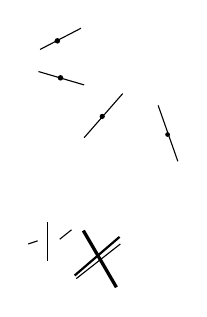
\begin{tikzpicture}[x=1cm,y=1cm]
\draw (0,1.55)--(.52,1.82); \fill (.22,1.66) circle (.035);
\draw (-.02,1.27)--(.56,1.10); \fill (.26,1.19) circle (.035);
\draw (.56,.43)--(1.05,.99); \fill (.79,.70) circle (.033);
\draw (1.5,.84)--(1.75,.13); \fill (1.62,.47) circle (.03);
\draw (-.15,-.92)--(-.03,-.88); \draw (.10,-1.13)--(.10,-.64);
\draw (.25,-.86)--(.40,-.74);
\draw[very thick] (.55,-.75)--(.97,-1.47);
\draw[thick] (.44,-1.32)--(1.01,-.83); \draw (.46,-1.36)--(1.02,-.92);
\end{tikzpicture}}

% margin note written sideways
\margin{$\begin{gathered}
x^{\unsure{2|3}}-y^{2}\\
\deleted{k(\unsure{x|x^{2}}}\\
\unsure{k|l}[\unsure{t|X}]\qquad \unsure{t|p}^{2},t^{3}\\
k[x,y]/xy
\end{gathered}$}

% letterhead
% Upside down relative to the archive number.
\begin{center}
INSTITUT\\
DES HAUTES ÉTUDES SCIENTIFIQUES\\
\rule{1cm}{0.4pt}
\end{center}

% archive sheet number: 131
